% \documentclass[conference]{IEEEtran}
\documentclass[a4paper]{article}
\usepackage{fancyhdr}
\usepackage{cite}
\usepackage{graphicx}
\usepackage[font=footnotesize]{subfig}
% \hyphenation{op-tical net-works semi-conduc-tor}

% 中文
\usepackage{fontspec}
\setromanfont{STSong}
%\setmonofont{Courier New}
\XeTeXlinebreaklocale "zh"
\XeTeXlinebreakskip = 0pt plus 1pt

\author{李合璧}

\begin{document}

\title{基于NDN网络的时间标签多层随机服务器同步算法}


% make the title area
\maketitle

% \thispagestyle{fancy}

\begin{abstract}
%\boldmath
作为新一代因特网架构,NDN网络提供了很多新的特性,使传统的IP网络的诸多缺点的得以克服。
群聊软件,如QQ群聊,视频会议等,需要保证群体中的每个人都能收到其他所有人所发布的消息。
传统因特网需要有一台中央服务器,收集每个人的消息,并推送给其他人。
这种结构存在严重的overhead,较长的实验,并且鲁棒性不强。
本研究课题充分利用NDN网络分布式的特点,并利用缓存和interest聚合实现数据同步的算法。
\end{abstract}

\section{概述}

即时多人聊天应用,例如qq,msn等热门应用,
所提供的关键功能是让群体中的每一个人都能向群体中发送消息,接受消息。
不同于两人聊天,多人聊天就涉及到如何让所有人都能收到其他人所发送的消息。
现阶段,此类应用都是运行在现有网络,即IP网络上的。这为其带来了不可避免的弊端。

IP网络被设计成点对点的通信,即通信过程中,整个网络层所知道的是通信源点和目标节点的IP地址。
路由器根据IP地址解析出下一跳的路径,并传递数据包。

在IP网络上,这些应用的同步算法是要有中央服务器的。每个人都和中央服务器建立连接。
中央服务器负责收集每个人的发送的消息,并将这些消息转发给其余所有人。
当一个参与者发送了一条文本信息,此信息会先经过路由到达中央服务器。
中央服务器维护了一个包含所有参与者的列表,
它收到消息后,经过计算处理,然后将此消息转发给需要它的人,以完成功能。

虽然这种办法可行,而且实际上在IP网络上也只能这样运行。
但是这种方法带来了严重的性能问题。

1. 存在大量的overhead
由于IP是点对点通信,这意味着中央服务器想要将一个消息传递给一个聊天室里的所有成员时,
不得不建立与所有人的TCP连接,并向每一个连接发送一份消息的副本。
如果有两个聊天用户在拓扑上非常近(例如他们连在同一个路由器上,而服务器可能在十跳之外。
这种情况下,需要两个相同的数据包,在这十个路由器上经过,而事实上只需要一个。
在群聊的环境中,用户量更大,更密集,从而造成更加大得多的overhead。

2. 鲁棒性不强
由于所有通信的实现都需要中央服务器的调节,这造成了单点故障。
如果服务器宕机了,或者被不法分子攻击,整个网络中的所有成员均不能正常通讯。
系统也无法自我修复,必须等到服务器维修好后才能重新上线服务。

IP的点对点的通讯模型导致了这些性能瓶颈,
而Named Data Network作为最近发展的一个新的网络架构,为解决这个问题提供了机会。
NDN的优于IP网络模型的根本点在于它不是点对点的模型。
NDN中,所有的资源使用一个独一无二的名字来索引,每个名字对应了一个资源。
资源获取是消费者主导的,也就是说,客户端想要访问一个资源时,
他以此资源的名字发送Interest数据包,并等待接受返回的数据。
由于资源是以名字来定义的,所有请求同一个资源的用户所发送的请求都是一样的:资源的独一无二的名字,
那么NDN中的路由器就会检测到相同的兴趣包,而不会将这个重复的兴趣包向下一跳传递。
当有内容返回时,NDN路由会将这个数据包向所有的端口转发,从而实现多路转发。
除此之外,NDN路由还涉及了缓存机制,当有内容数据包返回时,它会将这个包缓存在自己的内存中。
如果之后有用户请求相同的资源,NDN路由就会发现这个资源已经在自己的缓存中了,于是便可以直接返回给客户端。
这显著的减少了overhead,而且加快了数据包响应时间。

基于NDN的这些特性,它可以为即时多人聊天应用提供很好的架构基础,为解决这个性能瓶颈提供了新的机会。
利用这些特性,以上的问题可以得到较好的解决。
由于NDN的资源是有独特名字的,聊天室里的每一个人想要得到最新消息时,发送的兴趣包是相同的。
NDN路由会过滤掉所有重复的兴趣包,而往下一个路由只发送一份。
当数据返回时,内容包也会只有一份传递回来,并且由路由向各个端口分发数据包。
这样就实现了比传统IP方式小得多的overhead。
另一个方面,由于NDN不关心端点的IP,所有流量都是由Interest包的名字决定的,
因此可以将算法设计成分布式的,当有些节点出现故障,系统仍然可以继续工作,并且可以自我修复。

最近NDN研究人员提出了一种基于此的解决方案,ChronoSync。
这个方案是一个完全的分布式的算法,每一个用户都要定期向整个系统广播一个代表他自己当前状态的Interest。
任何人都可以回复这条Interest,只要他认识这个状态,而且他自己的状态更新。
在系统稳定时,每个人都会保留着其他人的Interest,
一旦自己有消息要发送,便立即响应这些Interest,从而将消息发布给团体里的所有人。

ChronoSync为此问题提供了很好的尝试和解决方案,也证明了比IP为基础的算法有明显的优势。
然而,这个算法仍有严重的不足。最大的问题在于,它是一个完全分布的算法,系统没有能力处理特殊情况。
例如,当有两个成员同时发布消息,他们都会响应所保留的别人发来的Interest。
然而,在NDN中,一个Interest只能带回一个数据包,这就必然导致有一个人的消息无法到达。
这样,系统就被分为两个不同阵营,各自有着不同的消息状态,互相无法识别。
更加糟糕的是,当系统里有很多人,出现这种情况的几率将会非常普遍,系统甚至会被分成若干个不同的阵营。
另外,ChronoSync的设计就决定了它无法扩展。每个人需要向全网广播兴趣包,来获取新的消息。
这样这个系统就只能在有限的小范围内使用,如果想在大范围内使用,就必须有分层机制,让复杂度指数递减。

在这种情况下,我们提出了TreeSync来解决此问题。我们的设计目标有以下几点:

1. 必须是分布式的。这样才能是系统更健壮,鲁棒性更强。
2. 有能力处理特殊情况,包括多个并发的消息。
3. 要能在大范围内进行扩展。

我主要完成的工作有:

1. 设计了TreeSync来解决NDN中即时多人聊天应用的信息同步问题。
2. 在ndnSIM中做了仿真。
3. 与ChronoSync做对比,证明算法的优越性。

接下来各章将会按照如下方式展开。在第二章,将会介绍NDN相关背景和其特性,为后文的算法描述做基础。
第三章,将会详细讨论算法的设计细节。第四章讨论现有的工作。第五章总结全文。

\section{NDN背景}

Named Data Network,简称NDN,是未来因特网架构的一部分。
该项目项目旨在开发一个新的互联网架构,可以对互联网目前的基于主机的,点至点的通信体系结构的和地址的弱点进行优化。
该项目研究并加以解决以下问题,以验证NDN作为未来互联网体系结构的技术挑战:
路由的可扩展性,快进,信任模型,网络安全,内容保护和隐私,以及基本的传播理论。
该NDN项目已于2010年9月资助的美国国家科学基金会NSF下的未来互联网体系结构项目的四个项目之一。
不同于现有的IP网络,NDN中不使用端到端的解决方案。

在NDN通信接收端,数据数据是由消费者驱动的。
接收数据时,消费者发出一个兴趣分组,它带有用于识别所需要的数据的名称。
例如,消费者可以请求`/ustc/video/a.mpg`。
路由器记得该请求进入的端口,然后在其转发的转发兴趣报列表(FIB )中查找名称。
它是通过填充一个基于名字的路由协议。
当兴趣包达到具有所请求的数据的节点时,一个数据包被发送回,
它带有两个名称和内容数据,与生产者的签名一起。
此数据包沿着兴趣分组的反向的路径,回到消费者。
需要注意的是,无论是兴趣包还是数据包,都不携带任何主机或接口地址(如IP地址)。
兴趣包路由到数据是基于兴趣包所包含的报文的名字,数据包产生者根据由兴趣包在每个路由器跳状态信息原路返回。
NDN路由器保持兴趣包和数据一段时间,作为缓存。
当多个相同兴趣包所请求的为同一个数据,那么只有第一个对数据源的兴趣包会向上游发送。
该路由器然后将这个转发信息存储在转发兴趣包表( PIT )中 ,
其中每个条目包含兴趣包名和一组从接口,这些接口都是发送该兴趣包来的接口。
当数据包到达时,路由器就会找到与之对应的PIT项和数据转发到所有列出的接口PIT的条目。
路由器然后删除相应的PIT表项,并将其缓存在自己的本地缓存中。
这使用路由器的缓冲存储器,并采用高速缓存替换策略。
数据有请求它的兴趣包的精确相同的路径,但是传输方向相反。
一个数据满足一个兴趣包,在每个跃点,实现逐跳流量平衡。
一个NDN数据包与其是来自何处,或在有可能被转发到的位置是独立的,
因此,路由器可以缓存它来满足未来的潜在需求。
这使NDN自动支持各种功能,而无需额外的基础设施,
包括内容分发(许多用户要求在不同的时间相同的数据),
多播(许多用户请求相同的数据在同一时间),
流动性(用户请求来自不同位置的数据),
并延迟容忍网络(用户有间歇连接)。
例如,考虑一个消费者在移动的车辆中观看流媒体视频。
消费者可以请求一些数据,但然后移动到一个新的本地网络。
虽然数据将在到达旧的位置和被丢弃,但是沿着路径会被缓存。
当消费者重发兴趣包,它可能会从附近的一个缓存中提取数据,使得中断最小。
数据缓存接近消费者提高网络传输性能,并减少对特定数据源的依赖。
这样就能有效避免由于故障或攻击可能导致的失败。

\section{相关工作}

\begin{figure}[!t]
\centering
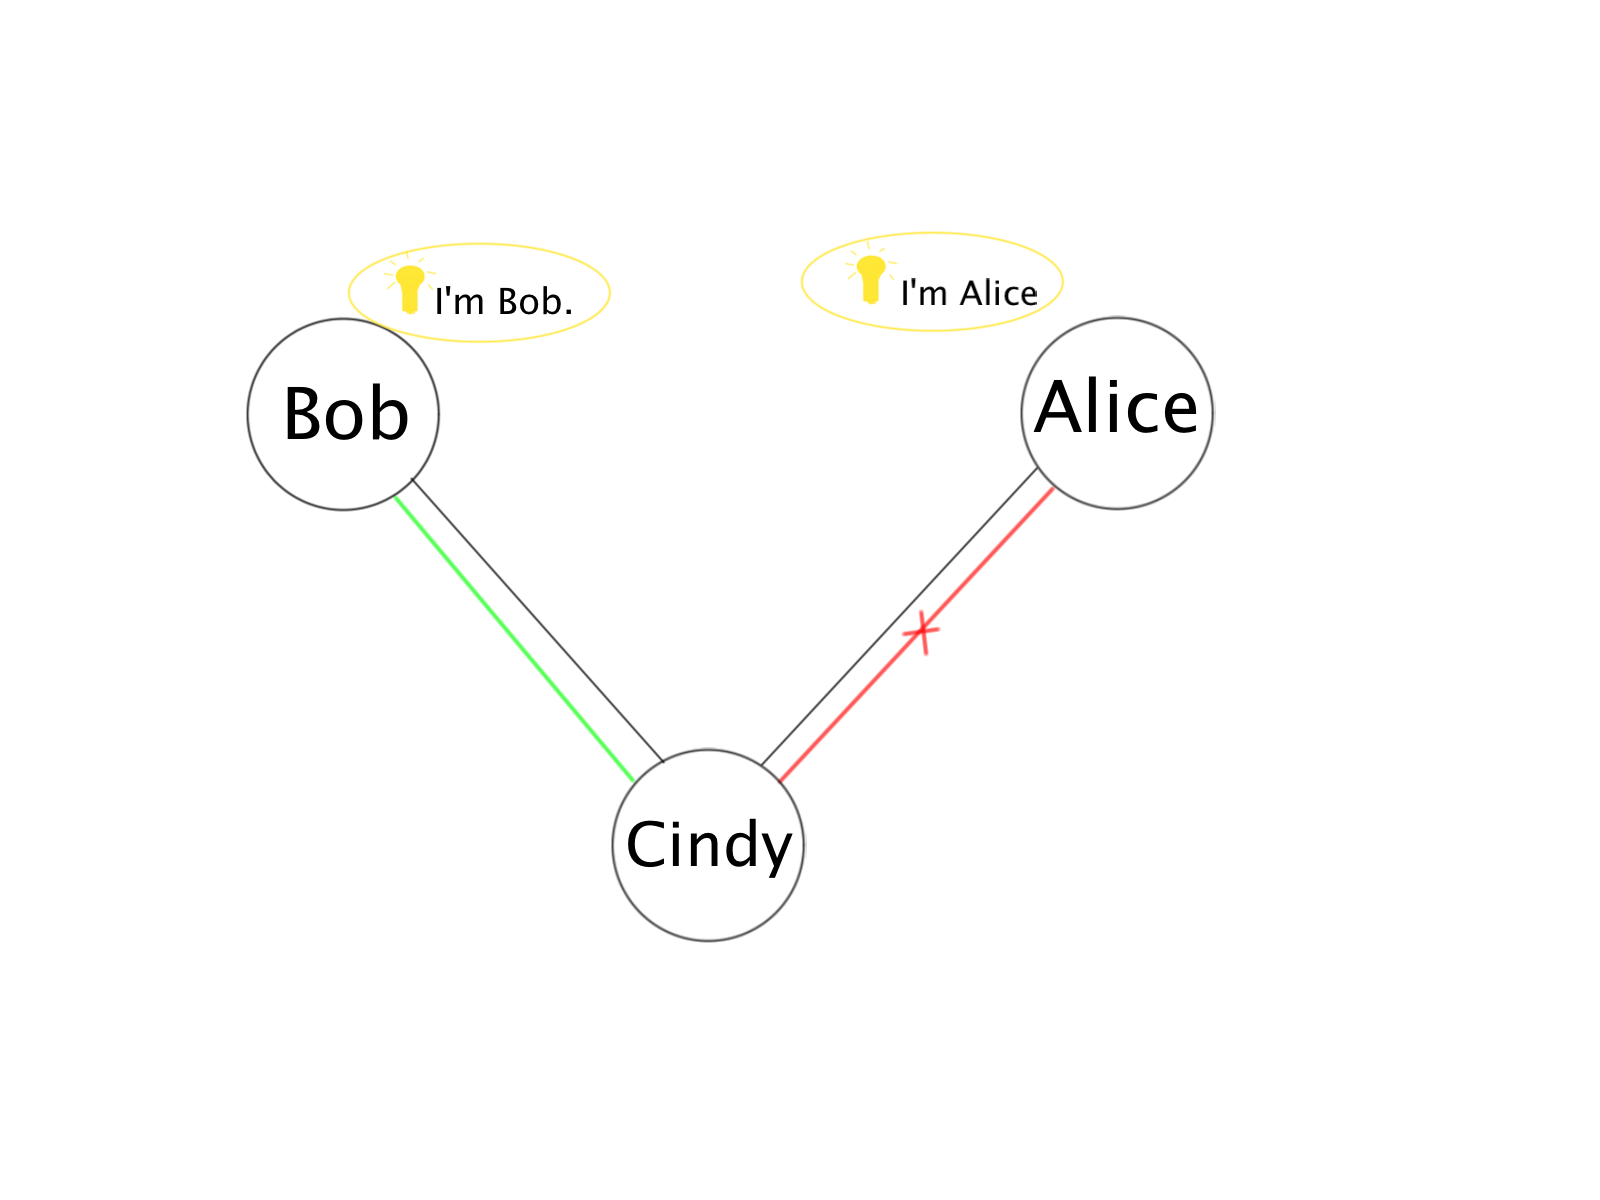
\includegraphics[width=3.5in]{../png/simultaneous.png}
\caption{Simultaneous Message Generation Problem on ChronoSync}
\label{simultaneous}
\end{figure}

这一章,我们主要讨论NDN平台中解决此问题的另一个方案:ChronoSync。
来自加州大学洛杉矶分校的Zhenkai Zhu最近提出了此方案。
这是一个完全分布式和服务器较少的协议。

任何ChronoSync的应用程序的核心是两个相互依存的组件。
同步的数据集的状态的ChronoSync模块,
和响应该数据集的状态的变化的应用逻辑模块。
在ChronoChat ,ChronoSync模块以一个摘要树的形式保持当前用户的所有邮件知识。
在一个摘要日志的形式的数据集的状态变化。
当ChronoSync模块发现聊天室有新的消息,它会通知ChronoChat逻辑模块来获取和存储的消息。

为了发现数据集的变化,ChronoSync模块向
每个ChronoChat实例发送一个同步的兴趣,
其名称中包含的状态摘要,并将此状态维持在根摘要树。
通常,通过摘要树和摘要日志的帮助,ChronoSync可以直接推断数据集的更改,
以及与包含数据回复到同步感兴趣的变化,这是称为同步数据。

Chronosync仅仅着眼于促进有关在数据集中的新数据项的同步,
具体知道了同步信息后做什么是应用程序的工作。
例如,在ChronoChat同步数据带回消息的名字新添加到聊天室,
因而使用者的知识该数据集是带来最新。
然而,用户可 决定是否要取回所有丢失的信息,或只取回最近期的。

ChronoSync的主要缺点是控制能力,其短,
导致的问题来处理频繁的同步数据的产生。
当这种情况发生时,系统将被分成两个不同的组,并且不能识别来自彼此消化。
例如,如图所示\ref{simultaneous}
Cindy发出同步的兴趣,要求谁产生一个最新的消息。
如果Alice和Bob说一些在接近的时间,也就是说,
Alice说些什么之前,Bob的话达到Cindy。
在这种方式下,爱丽丝将响应Cindy的同步兴趣,
但它永远不会达到Cindy因为从Cindy同步的兴趣只能取一个数据早在NDN 。
在这个时候,Bob和Cindy都在同一个状态,但Alice是没有的。
本系统被分为两个组,可以不相互识别。

\section{设计}

\subsection{设计概述}
在这小节中,我们将要简要讨论整个同步过程。后面的章节将会详细讲述同步的各个部分的细节。
1.树形拓扑
当有人要加入这个系统,他要做的第一件事就是在系统的拓扑中找到一个位置。
一般的,在最初阶段,每一个人都要找到自己的位置。
每个人会等待一个随机的时间,然后发送“Any Server Interest”请求。
如果他没有收到回复,他将会假设自己是控制器,所以能够去回复别人的“Any Server Interest”请求。
当收到这种回复时,参与者会将他所在节点的父节点设置为收到回复的发起者,并向他索要同步控制信息。
“Any Server Insterest”是和特定层级相关的,这是为多层树结构做准备。

每一个人都要发送心跳包来确定自己的控制节点是否还存在。
一旦检测到其控制节点宕机了,或者由于什么原因下线了,
一个新的控制器会从这个控制器所管辖的客户中选出一个,接替它的位子。
当然,一个新的参与者可以很容易的从他的附近找到一个节点当做自己的控制节点。

2.控制信息
控制器通过向自己的子节点发送控制信息来主导同步过程。
控制信息并不是真正的数据,而是一种包含什么时间在什么地方有新数据的信息包。
它会告诉接收者,应该在正确的时间到正确的地点拿取数据。
此包中除了包含真正消息的NDN名字,还包含一个标签。
当控制信息顺着拓扑树向下传播时,每一层的控制器都会将自己的名字和他当前的时间加入这个标签。
最终结果是,节点收到的控制信息包中将会包含它上层所有的控制器的名字和时间信息。

3.同步
当一个节点产生消息,或者更一般的,知道一些新的东西需要向群体中传递,他将会沿着拓扑树向上和向下传递。

向上传递。
当一个节点有新消息要发布,它想他的父节点,也就是他的控制器发送一个带有实际消息名称的Interest。
当控制器收到这个Interest,他将自己的名字和时间添加到这个记录的标签中,然后把它存储在自己本地的日志中。
如果他还有上层节点,它会按照同样的方式向上传递。

向下传递。
为了得到最新的控制信息,每一个用户都会定期向他的控制器发送同步兴趣包,我们称之为“Anything New Interest”。
该包中包含他所知道的最新的标签信息。当一个同步兴趣包超时了,用户会重发此兴趣包。
当控制节点收到该兴趣包后,会和自己的当前知道的最新的标签进行比较。
1.如果标签的时间和他自己的时间是一样的,说明现在他和客户的状态是相同的,此时不需要传递控制信息。
控制节点会把这个兴趣包保留,以便以后有新的信息时能够迅速响应。
2.如果这个标签比他自己的更早,说明该客户的状态已经旧了,需要更新。这时候,他会将用户标签时间点之后的所有新的记录返回给该用户。
当收到同步兴趣包的返回结果后,客户端会将这个消息记录在自己的日志中,并更新自己的状态。
这时候他的状态会比他保留的同步兴趣包新,所以会按照相同的方式,继续将此消息向他的子节点传递。
从而可以达到将控制信息转发给全局的目的。

4.实际消息本体的获取
当收到控制信息后,每个人都会知道新的消息的NDN名字。
他们直接发送数据请求兴趣包,去向消息产生者索取消息实体。
因为数据的名字在NDN中是唯一的而且稳定不变的,每个参与者的发送的索取相同信息的兴趣包是相同的,
那么这些兴趣包就会被路由聚集,并只发送一份兴趣包的拷贝去下一跳路由。
这就保证了每一个链路中相同的兴趣包只有一个,而不会有重复。当这个兴趣包达到消息产生者后,他会返回消息实体。
此数据包会沿着兴趣包相反的路径传递到所有发送兴趣包的用户,因此overhead非常小。
同时,返回的数据包可以被路由器缓存到本地的内存中,所以当之后有用户请求相同的数据,
他将会直接从临近的路由的缓存里面拿,而不是从消息的产生者那拿。

\begin{figure}[!t]
\centering
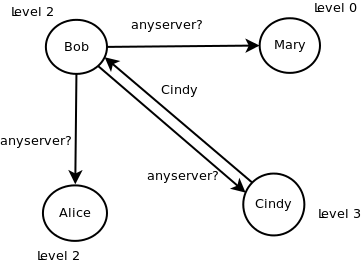
\includegraphics[width=2.5in]{../png/server-generation.png}
\caption{Server Generation}
\label{server_generation}
\end{figure}

\begin{figure*}[!t]
\centering
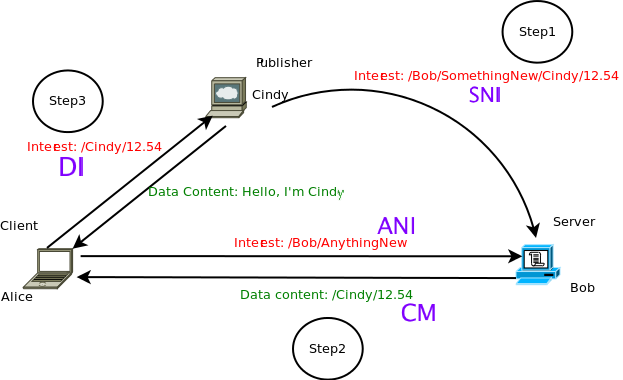
\includegraphics[width=4.5in]{../png/synchronization.png}
\caption{Synchronization and Data Fetching}
\label{synchronization}
\end{figure*}

\subsection{命名规则}

命名是NDN应用程序最重要的部分之一,因为NDN的本质是以名字命名数据。
在这一章,我们简要描述我们在设计中所使用的所有兴趣包的名字。
后面的章节将会分别详细讲述这些兴趣包的用途。

我们的设计中总共有四中兴趣包的名字。
Anything New Interest 用于产生控制器树形拓扑。
Something New Interest 和 Anything New Interest 用于控制消息的传输。
Data Interest 用来获取真正的消息实体。

名称的第一部分是为了保证路由可以正确的转发它们。
’/broadcast’的兴趣包会被路由到所有相关的端口。
’/serverName’和’/publisher’的兴趣包会被路由到指定的节点。

第二部分’/treesync’是标志当前应用程序的标签。

其他的成分是和具体流程相关的,我们将在后面几章分别讨论。

\subsection{树形拓扑产生}

为了产生控制器,我们将使用“Anything New Interest”。
名字的前两部分是为了路由传输和应用处理兴趣包。
第三个部分是兴趣包的类型。
最后一个元素“level”是一个数字,代表了当前这个兴趣包所使用的控制器层级。

在开始阶段,每个人都是独立的没有控制器的。
它们会各自等待一个随机的时间,然后向所有聊天用户广播一个ASI来询问周围有没有控制器。
然后他们会等待一个特定时间Ts。
如果能在Ts过期前收到返回的数据包,它就会将返回此包的用户作为他的父节点,然后发送给他同步兴趣包来索取控制信息。

如果他没有在Ts过期前收到回复,他就会将自己作为一个控制节点,并且准备好回复别的节点的相同的请求。
当区域很大时,在所有一级控制节点之上,会产生更高层的控制节点。
这些节点的生成和之前的算法一样,只是在等待时间上,会和其层级相关,更大的等待时间可以生成更大的区域。
如果在到期之前没有收到回复,控制器就将自己的层级加一。

我们设置一个小的整数,作为最高层级。
只要一个参与者没有上层控制器,而且自己不是最高层控制器,他就会进行这个产生过程。
如果一个节点已经有控制节点,他会向该节点定期发送心跳兴趣包来检测该节点的有效性。
我们将在第七节讨论节点宕机的处理。

注意到控制节点的产生过程和实际拓扑是息息相关的,信息传递的方向当然也是和拓扑相关的。
这就使得经过控制器的延迟不会比直接传递的延迟有显著的增加。
从而保证了传输时延性能。

\begin{figure*}[!t]
\centering
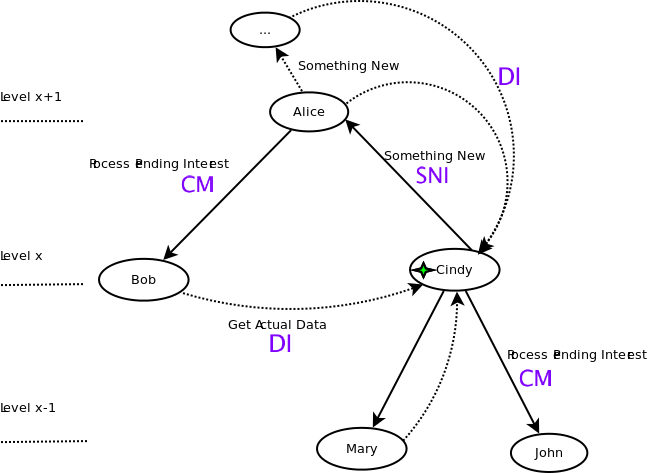
\includegraphics[width=4.5in]{../png/tree-synchronization.png}
\caption{Multi-Level Synchronization}
\label{tree_synchronization}
\end{figure*}

\subsection{同步过程}

本章,我们将描述在系统中到底是如何同步的。
如图所示,子节点向其父节点发送SNI来通知他有一个新的消息。
控制节点然后会回复他保存的待决定的ANI,其中包含这个新的消息。
参与者通过分布式的方式获取消息实体。图4显示了多层拓扑的同步。
每个节点都会通过发送SNI和满足ANI来向上和向下传递控制信息。

1.Something New Interest。
当一个节点产生一个新的消息,或者他收到来自下层节点的SNI,他会将此消息向上传递给自己的控制节点。

当一个参与者产生一个新的数据,他将会做下面这些事:
1.添加这个数据进入自己本地的数据存储器
2.将自己的标签加入这条记录中,并且将这条记录放入自己的记录存储器。
3.向他的控制节点发送SNI,其中包含他的标签和实际数据的NDN名字。
4.处理来自子节点的待处理的ANY

注意到SNI在其后面包含了真是的数据名字,所以当控制节点收到此SNI后,他可以立即将这个消息向上或者向下传递。

2.Anything New Interest。
为了得到控制信息,每一个节点都会周期性的向他的控制节点发送带有他当前最新标签的ANI。
当一个控制节点收到这个兴趣包时,他会将其中包含的标签信息和他自己的最新标签做对比。
有如下三种情形:
1.此标签和他自己的标签时间相同。
这时候,他将会把这个兴趣包保留为待处理的同步兴趣包,这样能够在他有状态变化时第一时间将此变化回复给其客户端。
2.收到的兴趣包中包含的标签晚于自己当前的标签。
这时候,他比较这个记录的时间,找到本地记录中所有比此标签新的记录,然后将所有记录返回给该兴趣包。
3.在自己的记录中没有此标签对应的用户信息。
这种情况下,需要将所有的记录都发送给子节点。

当子节点收到ANI的数据包时,他会做如下的事:
1.将记录从数据中提取出来
2.更新自己当前的记录存储器
3.处理待处理的同步兴趣包
4.发送兴趣包以获取消息实体

一般的,控制器控制着其内部的同步,所以其所有的子节点都会有这个控制器的标签信息。
所以大部分情况下,组内的节点只需要将他的父节点的控制信息包含在ANI中皆可以完成同步。
当这个系统处于稳定状态,所有的节点都发送相同的ANI,这些ANI是可以被NDN路由器聚合的。
而数据又是通过相反的路径精确的到达每个参与者。
当一个节点移动到另一个组内,或者控制器宕机或下线了,该节点将会找到一个新的控制器。
这种情况下,使用他先前的控制器的标签就不行了。
这种情况下,他将自己知道的所有标签发送给新的控制器。
这种模型的设计可以提供天然的对于鲁棒性和移动性的支持,我们将在第八节讨论。

\subsection{消息本体获取}

服务节点所同步的是消息的名称。

节点得知正确的内容所在的地址(其名称)后,直接向这个地址发interest获取消息本体。

使用了NDN的缓存和interest聚合。好处。

\subsection{鲁棒性和移动性支持}

\begin{figure*}[!t]
\centering
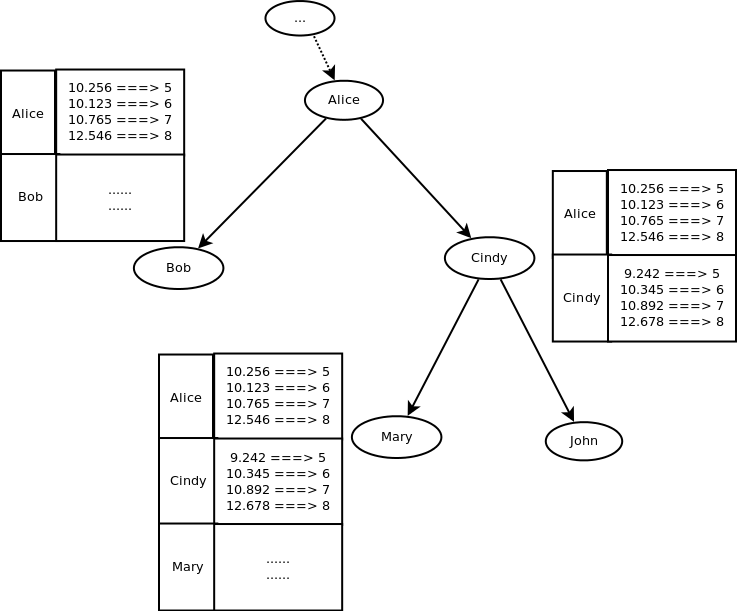
\includegraphics[width=4.5in]{../png/mobility.png}
\caption{Robustness and Mobility Support}
\label{mobility_pic}
\end{figure*}

鲁棒性:当一个节点下线后,如何从他的子结点中选出一个代替他。

移动性:当一个节点移动后,其上层节点很有可能共享同一个上层节点。所以还是可以使用其时间标签正常同步。

\subsection{特殊情况分析}

\begin{figure}[!t]
\centering
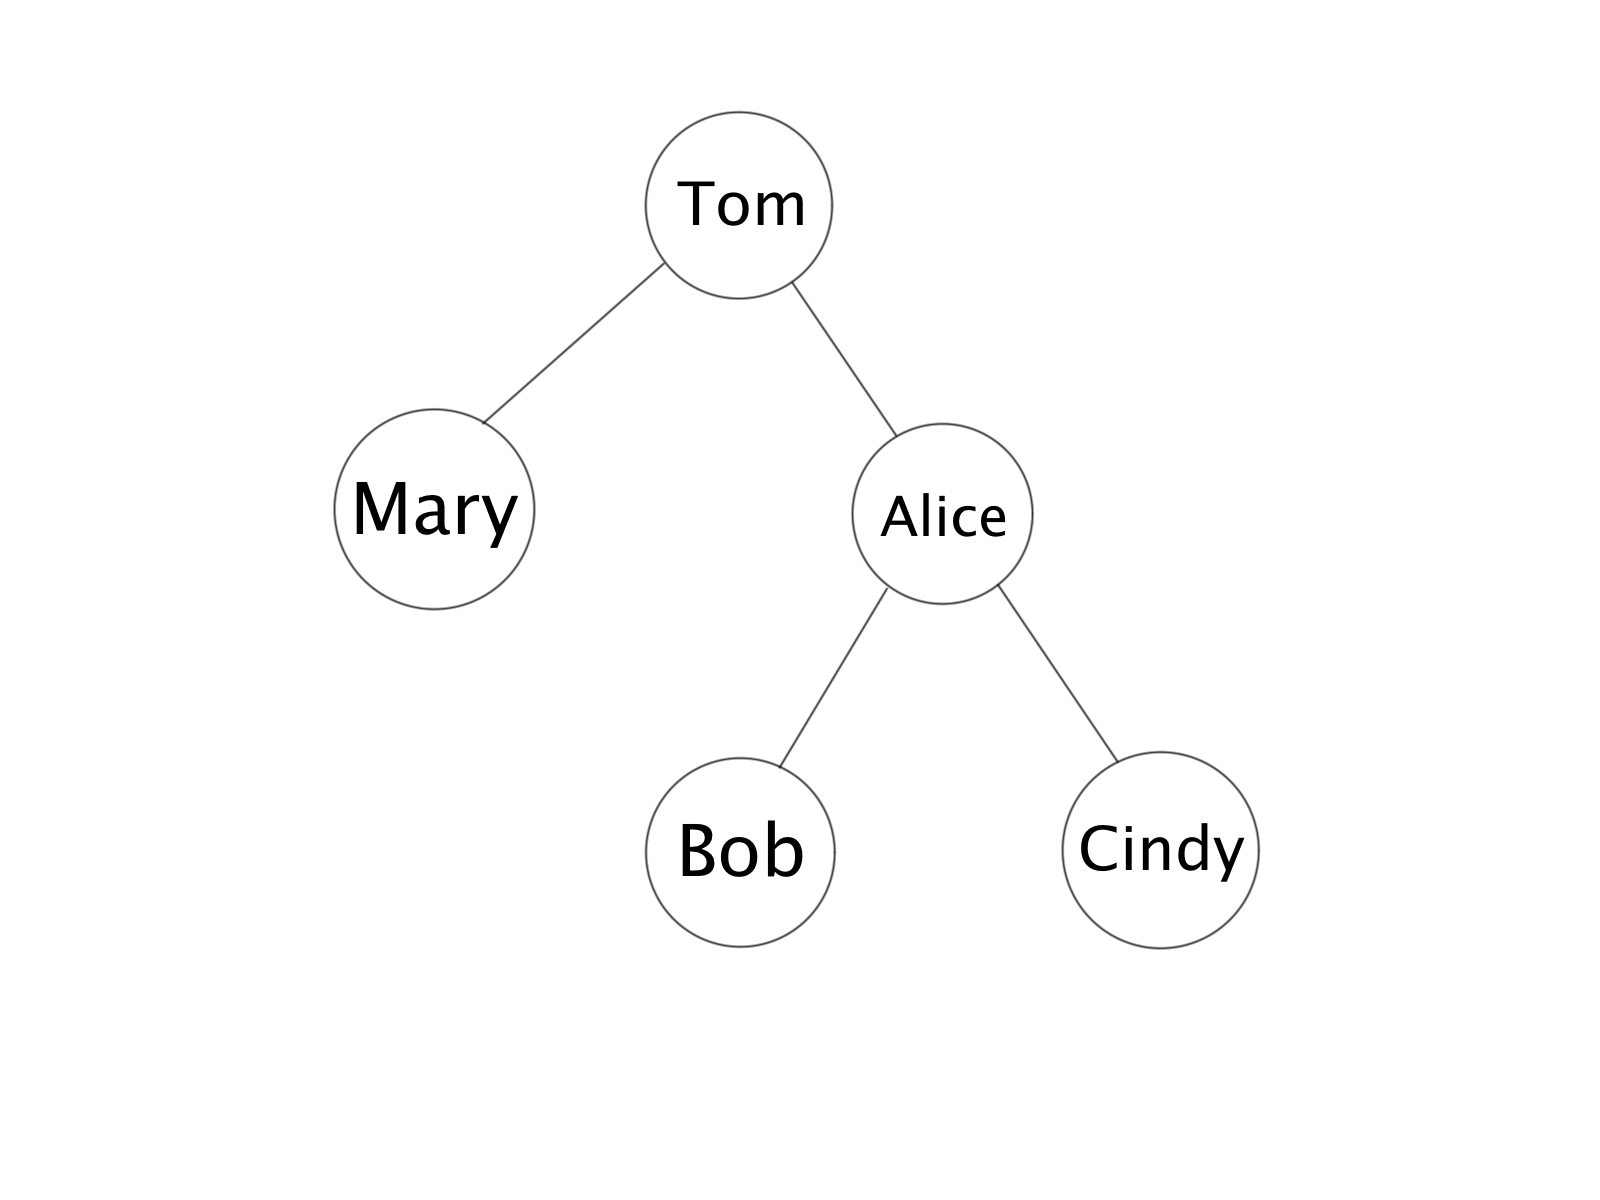
\includegraphics[width=2.5in]{../png/merit.png}
\caption{Handling Simultaneous Message Generation}
\label{merit}
\end{figure}

\section{仿真}
\subsection{概述}

\begin{figure}[!t]
\centering
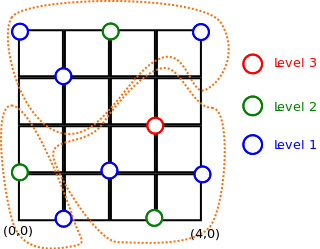
\includegraphics[width=2.5in]{../png/paper-topo.png}
\caption{5x5 Grid Topology and Generated Servers}
\label{paper_topo}
\end{figure}

我们在ndnSIM上实现了TreeSync的仿真。
ndnSIM是Network Simulation(NS3)的一个模块,用于提供一个NDN的IP层的包装。
作为对比,我们同样实现了一个ChronoSync的ndnSIM版本。
在这一章中,我们首先验证逻辑的正确性和功能的实现。
然后我们在overhead和传输时延上做评估。

使结果更具一般性,我们采用5x5的网格拓扑结构。
网格中的每一个节点都代表一个参与者,所以总共更有25个节点。
拓扑图可能看起来很简单,但是实际上它包含6种不同环境中的节点,最大8跳的路由。
我们认为这个拓扑可以很好的代表一个一般的脱兔结构。
树形拓扑按照之前描述的算法生成。
所有的链路都具有10ms的延迟和1Mbps的带宽。
我们让参与者随机的生成新的数据,并且我们改变他们生成数据的频率来研究变化趋势。
每个人产生信息的周期是独立的。

\subsection{功能实现}

\begin{figure}[!t]
\centering
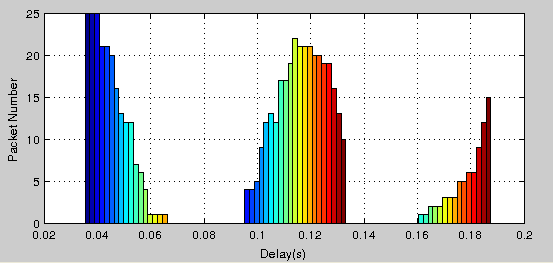
\includegraphics[width=2.5in]{../png/function-delay.png}
\caption{Delay for every node to receive data}
\label{function_delay}
\end{figure}

1.控制节点产生。
在网格拓扑中,控制节点产生像预期一样工作。
产生了一个四层的拓扑,最高级的控制节点在节点(3,2)上。

2.消息同步。
所有的消息都能够成功的传递给聊天室的所有人,不会丢失任何消息。
图8显示了当产生频率为2/7Hz时的时延。从图中可以看出,时延被分为三个部分。
很快,平均,和稍慢。这是和树形拓扑紧密相关的。
如果接收者在消息产生者很近的位置,他们在树形拓扑中也会距离很近,这样他就能够很快得到控制信息,进而获取实际消息实体。
然而,当两个参与者在树形拓扑中相距很远时,控制信息要跨越好几个层级才能到达,导致了相对更大的时延。


\subsection{效果评估}

\subsubsection{链路负载}

\begin{figure}[!t]
\centering
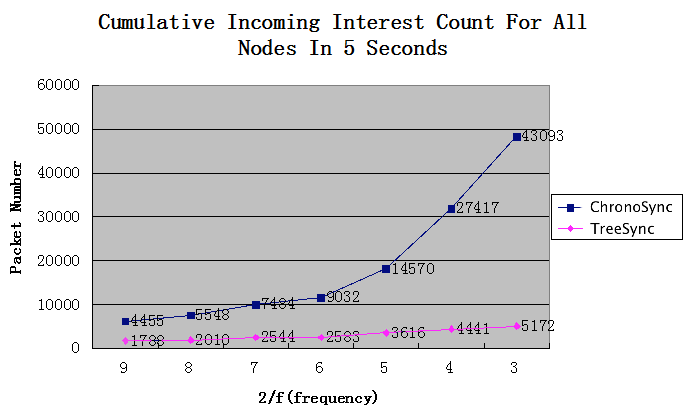
\includegraphics[width=2.5in]{../png/all-incoming-interest-revised.png}
\caption{Incoming Interest Count for All the Nodes}
\label{overhead}
\end{figure}
\begin{figure}[!t]
\centering
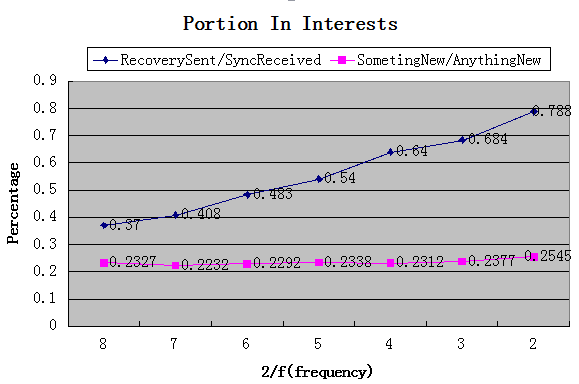
\includegraphics[width=2.5in]{../png/portion-in-interests.png}
\caption{Portion in Interests}
\label{recovery_percentage}
\end{figure}

我们的设计在控制性上面有很大的优势,所以在overhead上会比ChronoSync有显著的减少。
在我们的试验中,我们改变消息声称的平率,然后观察overhead的变化。
在图9种,当频率增加时,我们的设计在包数统计上会有线性的增加,然而ChronoSync却遭受了指数的增长。
这是因为当产生消息的频率增加时,同时产生消息的频率也指数增加,那么ChronoSync就必须发送额外的恢复兴趣包来处理这种冲突。
注意到我们使用的是所有进入的兴趣包的数目统计,因为它可以代表整个状态。
NDN路由器的聚合性也可以减少进入的兴趣包数。
从图10可以看出,在ChronoSync中节点需要发送恢复兴趣包的比例随着频率增长得非常快,然而在我们的设计中,SNI和ANI的比例基本保持不变。

\subsubsection{延迟}

\begin{figure}[!t]
\centering
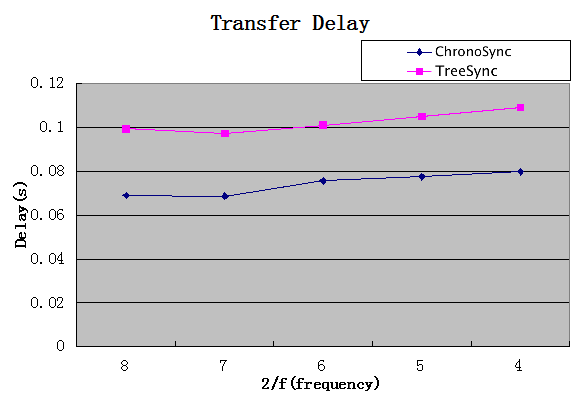
\includegraphics[width=2.5in]{../png/delay-compare-revised.png}
\caption{Delay Compare}
\label{delay_compare}
\end{figure}

\begin{figure}[!t]
\centering
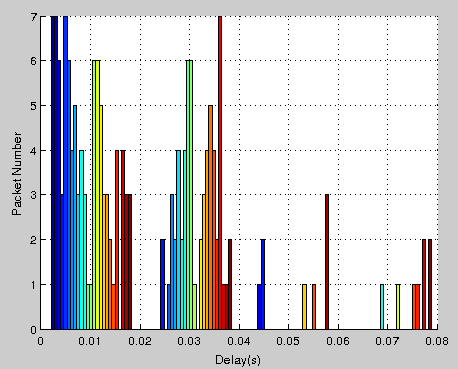
\includegraphics[width=2.5in]{../png/data-fetch-delay.png}
\caption{Data Fetching Delay}
\label{data_fetch_delay}
\end{figure}

由于控制信息要经过多层控制器,即时拓扑结构和实际拓扑是紧密相关的,延迟效果依然比完全按照最有路径的ChronoSync稍差。
但是,当数据产生更加频繁时,ChronoSync需要发送更多的恢复兴趣包,并且当带宽不足时会增加其时延。
如图11所示,TreeSync的时延要稍大于ChronoSync,但是仍然很好,并且两种方法都大幅度优于IP网络模型解决方案。
考虑到获得的巨大的控制性能,这种权衡牺牲是值得的。

另一点,在我们的数据中,实际数据的获取是完全分布式的,可以充分利用NDN结构的优点。
图12显示了参与者从发送实际消息请求到得到数据的延迟,可以看到这个过程非常迅速。
并且这种设计也为低时延和小overhead做出了贡献。

\section{总结}

在这篇论文中,我们提出了基于NDN网络的解决即时多人聊天应用的新的算法,TreeSync。
TreeSync充分利用了传统中央服务器式模型和NDN的有效的分布式特性。

首先,多层控制节点可以提供强大的控制能力,来处理复杂的情形。
其次,该设计的本质的分布式特征让它能够有效率的获取消息,并且具有鲁棒性和移动性支持,享有极小的overhead。
另外,树形结构的层级设计也为扩展性提供了保证。当节点增多时,复杂度是指数下降的。

我们在ndnSIM上实现了TreeSync,并且评估了其性能。消息能够正确而快速的在群体中相互同步。
在拥有较快同步时延的同时,overhead相对于其他算法有显著的降低。

\begin{thebibliography}{1}

\bibitem{FIA}
``NSF Future Internet Architecture Project'', http://www.nets-fia.net
\bibitem{NDN001}
Zhang, L., Estrin, D., Burke, J., Jacobson, V., Thornton, J. D., Smetters, D. K., ... \& Yeh, E. (2010).
Named data networking (ndn) project. Relatório Técnico NDN-0001, Xerox Palo Alto Research Center-PARC.
\bibitem{ChronoSync}
Zhu, Z., \& Afanasyev, A. (2013).
Let’s ChronoSync: Decentralized Dataset State Synchronization in Named Data Networking.
In Proceedings of the 21st IEEE International Conference on Network Protocols (ICNP 2013).
\bibitem{ndnSIM}
Afanasyev, A., Moiseenko, I., \& Zhang, L. (2012).
ndnSIM: NDN simulator for NS-3. University of California, Los Angeles, Tech. Rep.
\bibitem{ns3}
``ns-3: a discrete-event network simulator for Internet systems.'', http://www.nsnam.org
\bibitem{OSPF}
Moy, J. (1998). Open shortest path first (ospf) version 2. IETF: The Internet Engineering Taskforce RFC, 2328.
\bibitem{OSPFN}
Wang, L., Hoque, A. K. M. M., Yi, C., Alyyan, A., \& Zhang, B. (2012).
OSPFN: An OSPF based routing protocol for Named Data Networking.
University of Memphis and University of Arizona, Tech. Rep.
\end{thebibliography}

\end{document}
